\documentclass{standalone}
\usepackage{tikz}
\usepackage{xcolor}
\usetikzlibrary{decorations.pathreplacing}

\colorlet{samplecol}{green!80!black}
\colorlet{unlatentcol}{blue!90!white}
\colorlet{latentcol}{red}
\colorlet{sminusucol}{cyan}

\begin{document}
	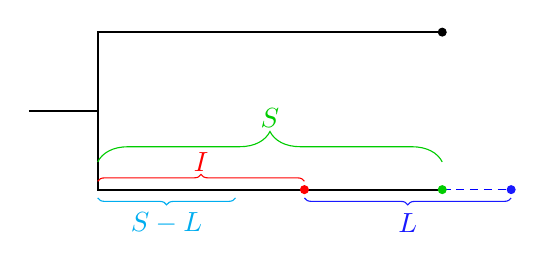
\begin{tikzpicture}[xscale=1.75]
		\coordinate (root) at (0, 0);
		\coordinate (branch) at (.5, 0);
		\coordinate (up) at (.5, 1);
		\coordinate (upsample) at (3, 1);
		\coordinate (down) at (.5, -1);
		\coordinate (sample) at (3, -1);
		\coordinate (latent) at (2, -1);
		\coordinate (unlatent) at (3.5, -1);
		\coordinate (sminusu) at (1.5, -1);
		\draw[thick] (root) -- (branch) (upsample) -- (up) -- (down) -- (sample);
		\draw[densely dashed, color=blue] (sample) -- (unlatent);
		\draw node at (sample) [shape=circle, draw, fill=samplecol, color=samplecol, inner sep=1pt] {}
		node at (latent) [shape=circle, draw, fill=latentcol, color=latentcol, inner sep=1pt] {}
		node at (unlatent) [shape=circle, draw, fill=unlatentcol, color=unlatentcol, inner sep=1pt] {}
		node at (upsample) [shape=circle, draw, fill=black, color=black, inner sep=1pt] {};
		\draw[decorate, decoration={brace, raise=3pt}, color=latentcol] (down) -- node [yshift=10pt] {$I$} (latent);
		\draw[decorate, decoration={brace, raise=10pt, amplitude=11pt}, color=samplecol] (down) -- node [yshift=26pt] {$S$} (sample);
		\draw[decorate, decoration={brace, mirror, raise=3pt}, color=unlatentcol] (latent) -- node [yshift=-12pt] {$L$} (unlatent);
		\draw[decorate, decoration={brace, mirror, raise=3pt}, color=sminusucol] (down) -- node [yshift=-12pt] {$S - L$} (sminusu);
	\end{tikzpicture}
\end{document}